\documentclass[tikz,border=5pt]{standalone}

\usepackage{tikz}
\usepackage{amsmath}
\usepackage{amsfonts}

\usetikzlibrary{arrows.meta,positioning,shapes.geometric}

\begin{document}
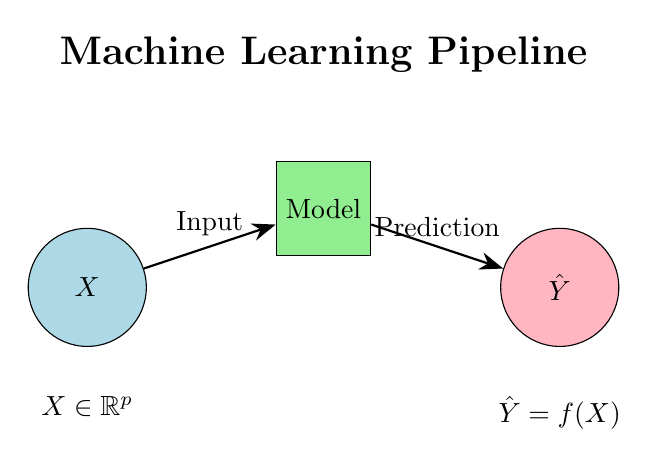
\begin{tikzpicture}
    % Define colors
    \definecolor{lightblue}{RGB}{173,216,230}
    \definecolor{lightgreen}{RGB}{144,238,144}
    \definecolor{lightpink}{RGB}{255,182,193}
    
    % Draw nodes
    \node[circle, fill=lightblue, draw, minimum size=1.5cm] (A) at (0,0) {$X$};
    \node[rectangle, fill=lightgreen, draw, minimum size=1.2cm] (B) at (3,1) {Model};
    \node[circle, fill=lightpink, draw, minimum size=1.5cm] (C) at (6,0) {$\hat{Y}$};
    
    % Draw arrows
    \draw[-{Stealth[length=3mm]}, thick] (A) -- (B) node[midway,above] {Input};
    \draw[-{Stealth[length=3mm]}, thick] (B) -- (C) node[midway,above] {Prediction};
    
    % Add title
    \node[above=1cm of B] {\Large \textbf{Machine Learning Pipeline}};
    
    % Add mathematical notation
    \node[below=0.5cm of A] {$X \in \mathbb{R}^p$};
    \node[below=0.5cm of C] {$\hat{Y} = f(X)$};
\end{tikzpicture}
\end{document}